\documentclass[10pt]{beamer}
\usetheme{Madrid}
\usecolortheme{default}
\usepackage{algorithm}
\usepackage{algorithmicx}
\usepackage{algpseudocode}
\usepackage{amsmath}
\usepackage{amsthm}
\usepackage{amssymb}
\usepackage{multirow}
\usepackage{array}
\usepackage{tikz}
\usetikzlibrary{positioning,shapes.geometric, arrows, decorations.pathreplacing}
\usepackage[margin=3cm]{geometry}
\usepackage{titlesec}
\usepackage{hyperref}
\usepackage{booktabs}
\usepackage{biblatex}
\usepackage{amsfonts}
\usepackage{amssymb}
\usepackage{graphicx}
\usepackage{tikz}
\usepackage{booktabs}
\usepackage{tabularx}
\usepackage{array}
\usepackage{xcolor}
\usepackage{colortbl} % For cell coloring
\addbibresource{references.bib}
\graphicspath{{images/}}

% TikZ styles
\tikzstyle{process} = [rectangle, rounded corners, minimum width=3cm, minimum height=1cm, text centered, draw=black, fill=red!30]
\tikzstyle{arrow} = [thick,->,>=stealth]
\tikzstyle{io} = [trapezium, trapezium left angle=70, trapezium right angle=110, minimum width=3cm, minimum height=1cm, text centered, draw=black, fill=blue!30]
\tikzstyle{decision} = [diamond, aspect=2, minimum width=3cm, minimum height=1cm, text centered, draw=black, fill=green!30]
\tikzstyle{data} = [cylinder, shape border rotate=90, aspect=0.2, minimum height=1.5cm, text centered, draw=black, fill=orange!30]

\usepackage{graphicx}
\usepackage{amsmath}
\usepackage{booktabs}
\usepackage{array}

\title{BioMoQA Classifier}
\subtitle{Transformer-Based Classification for Island Biodiversity Literature}
\author{Léandre Catogni}
\institute{BiTeM Group - HES-SO Geneva \\ University of Geneva}
\date{\today}

\begin{document}

\frame{\titlepage}

\begin{frame}{Context \& Motivation}
\begin{itemize}
    \item \textbf{Challenge}: Exponential growth of scientific publications
    \item Researchers struggle to find relevant literature efficiently
    \item Manual literature review becomes impractical
    \item \textbf{Need}: Automated literature triage systems
\end{itemize}

\vspace{0.5cm}
\textbf{BiTeM Group Mission:} Enhance access to biodiversity literature through AI-powered analytical services
\end{frame}

\begin{frame}{Objectives}
\textbf{Build classifiers for 2 datasets:}

\begin{enumerate}
    \item \textbf{BioMoQA Dataset} (Giorgia's team)
    \begin{itemize}
        \item Manually labeled by domain experts
        \item Binary classification / ranking task
        \item Focus: Island ecosystem relevance
    \end{itemize}
    
    \item \textbf{IPBES Dataset}
    \begin{itemize}
        \item 3 labels corresponding to different subjects
        \item Multi-label classification
        \item "Super positives" of particular interest
    \end{itemize}
\end{enumerate}
\end{frame}

\begin{frame}{BioMoQA Data Analysis}

\textbf{Class Imbalance Problem:}
\begin{itemize}
    \item 326 positives (relevant)
    \item 123 negatives (irrelevant)
    \item Insufficient negatives for robust training/testing
\end{itemize}

\vspace{0.3cm}
\textbf{Solution:} Add synthetic negatives from PubMed
\begin{itemize}
    \item Publications post-2021 only
    \item Exclude island-related terms
    \item 1,000 additional negatives
\end{itemize}
\end{frame}

\begin{frame}{BioMoQA Data Analysis}
\begin{figure}
    \centering
    \includegraphics[scale=0.5]{images/class_distribution.png}
    \caption{Data types distrbituion}
    \label{fig:enter-label}
\end{figure}
    
\end{frame}

\begin{frame}{Data Content Analysis}
\begin{center}
\includegraphics[width=0.8\textwidth]{images/wordcloud.png}
\end{center}
\textbf{Key terms:} Geography, species, ecological concepts consistent with island biodiversity
\end{frame}

\begin{frame}{Workflow}
\begin{center}

\begin{figure}[h!]
    \centering
    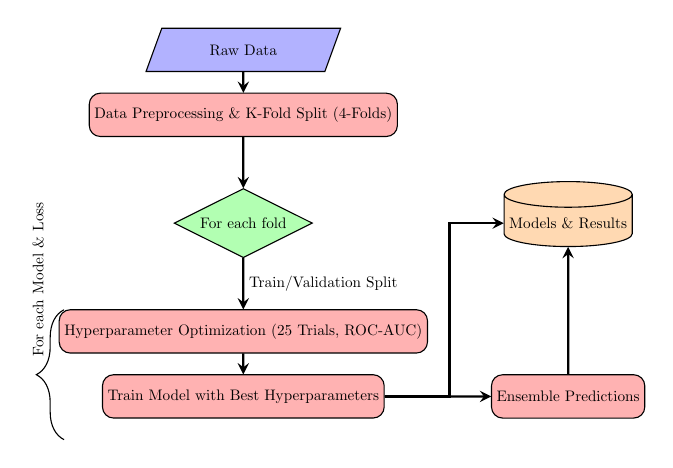
\begin{tikzpicture}[node distance=1.5cm, scale=0.55, transform shape]
        \node (start) [io] {Raw Data};
        \node (preprocess) [process, below of=start] {Data Preprocessing \& K-Fold Split (4-Folds)};
        \node (loop) [decision, below of=preprocess, yshift=-1cm] {For each fold};
        \node (hpo) [process, below of=loop, yshift=-1cm] {Hyperparameter Optimization (25 Trials, ROC-AUC)};
        \node (train) [process, below of=hpo] {Train Model with Best Hyperparameters};
        \node (ensemble) [process, right of=train, xshift=6cm] {Ensemble Predictions};
        \node (data) [data, right of=loop, xshift=6cm] {Models \& Results};
        
        \draw [arrow] (start) -- (preprocess);
        \draw [arrow] (preprocess) -- (loop);
        \draw [arrow] (loop) -- node[right] {Train/Validation Split} (hpo);
        \draw [arrow] (hpo) -- (train);
        \draw [arrow] (train.east) -- ++(1.5,0) |- (data);
        \draw [arrow] (train) -- (ensemble);
        \draw [arrow] (ensemble) -- (data);
        
        \draw [decorate,decoration={brace,amplitude=10pt},xshift=-4pt,yshift=0pt]
        (-4,-9) -- (-4,-6) node [black,midway,xshift=-0.6cm,yshift=2.2cm,rotate=90] {For each Model \& Loss};
    \end{tikzpicture}
    \caption{Experimental workflow for model training and evaluation.}
    \label{fig:workflow}
\end{figure}
\end{center}
\end{frame}

\begin{frame}{WorkFlow}
\begin{enumerate}
    \item Data preprocessing \& 4-fold cross-validation
    \item Hyperparameter optimization (25 trials, ROC-AUC)
    \item Model training with best parameters
    \item Ensemble predictions
\end{enumerate}
    
\end{frame}

\begin{frame}{Data Preparation}
\textbf{Cross-validation strategy:}
\begin{itemize}
    \item 4-fold CV on original 449 documents
    \item Each fold: 20\% test, 60\% train, 20\% dev
    \item Synthetic negatives added to train sets only
    \item Evaluation exclusively on expert-labeled data
\end{itemize}

\vspace{0.5cm}
\textbf{Why not 5-fold?}
\begin{itemize}
    \item Computational cost vs. benefit trade-off
    \item 4 folds sufficient for robust evaluation
\end{itemize}
\end{frame}

\begin{frame}{Pre-trained Models}
\begin{table}
\centering
\caption{Transformer models comparison}
\resizebox{\textwidth}{!}{%
\begin{tabular}{llcc}
\toprule
\textbf{Model} & \textbf{Domain} & \textbf{Parameters} & \textbf{Pre-training Data} \\
\midrule
BERT-base & General & 110M & BookCorpus + Wikipedia \\
RoBERTa-base & General & 125M & BERT data + additional text \\
BioBERT-v1.1 & Biomedical & 110M & BERT + PubMed + PMC \\
BiomedBERT-abstract & Biomedical & 110M & PubMed abstracts only \\
BiomedBERT-fulltext & Biomedical & 110M & PubMed + PMC full-text \\
\bottomrule
\end{tabular}%
}
\end{table}
\end{frame}

\begin{frame}{Fine-tuning}
\textbf{Training process:}
\begin{itemize}
    \item Fine-tune entire model on train set
    \item Address class imbalance with 2 loss functions
    \item Early stopping on dev set (patience = 3)
\end{itemize}

\vspace{0.5cm}
\textbf{Loss Functions:}
\begin{align}
\mathcal{L}_{\text{BCE}} &= -[y \log(\hat{y}) + (1-y) \log(1-\hat{y})] \\
\mathcal{L}_{\text{Focal}} &= -[\alpha_t (1-\hat{y}_t)^\gamma \log(\hat{y}_t)]
\end{align}

\textbf{Spoiler:} BCE performed better!
\end{frame}

\begin{frame}{Evaluation Metrics}
\textbf{Key formulas:}
\begin{align}
\text{Precision} &= \frac{TP}{TP + FP} \\
\text{Recall} &= \frac{TP}{TP + FN} \\
\text{F1} &= \frac{2 \times \text{Precision} \times \text{Recall}}{\text{Precision} + \text{Recall}} \\
\text{Cohen's } \kappa &= \frac{p_o - p_e}{1 - p_e} \\
\text{ROC-AUC} &= \int_{0}^{1} \text{TPR}(\text{FPR}) \, d\text{FPR}
\end{align}

\textbf{Kappa:} Agreement beyond chance | \textbf{AUC:} Ranking quality
\end{frame}

\begin{frame}{Hyperparameter Optimization}
\textbf{Strategy:}
\begin{itemize}
    \item F1-score threshold optimization on dev set
    \item 25 trials using random search
    \item Optimize for ROC-AUC (ranking focus)
\end{itemize}

\vspace{0.5cm}
\textbf{Optimized parameters:}
\begin{itemize}
    \item Learning rate (1e-5 to 5e-5)
    \item Positive class weight (BCE)
    \item Alpha \& gamma (Focal Loss)
    \item Weight decay (regularization)
\end{itemize}
\end{frame}

\begin{frame}{Results - Model Performance}
\begin{center}
\includegraphics[scale=0.4]{images/box_plot_kappa.png}
\end{center}

\end{frame}

\begin{frame}{Results - Model Performance}
\begin{center}
\includegraphics[scale=0.4]{images/box_plot_roc_auc_with_title.png}
\end{center}

\end{frame}


\begin{frame}{Results - Model Performance}
\textbf{Key findings:}
\begin{itemize}
    \item Domain-specific models slightly outperform general models on kappa score but not for ROC AUC
    \item BCE consistently better than Focal Loss
    \item Ensemble achieves best performance (ROC-AUC: 0.826)
\end{itemize}
\end{frame}

\begin{frame}{Results - Best Performance}
\begin{center}
\includegraphics[scale=0.3]{images/best_roc.png}
\end{center}
\textbf{Ensemble BCE:} ROC-AUC = 0.826, F1 = 0.879
\end{frame}

\begin{frame}{Statistical Testing}
\begin{center}
\includegraphics[width=0.9\textwidth]{images/nemenyi.png}
\end{center}
\textbf{Friedman test + Nemenyi post-hoc:}
\begin{itemize}
    \item Significant differences between model groups (p < 0.05)
    \item Clear performance hierarchy established
    \item Better performance when considering the title
\end{itemize}
\end{frame}

\begin{frame}{Ablation Studies}
\textbf{Title inclusion:}
\begin{itemize}
    \item Title + Abstract vs. Abstract only
    \item 2-3\% F1-score improvement with titles
    \item Titles provide crucial semantic signals
\end{itemize}

\vspace{0.5cm}
\textbf{Synthetic negatives:}
\begin{itemize}
    \item Compared 0, 500, 1000 additional negatives
    \item 1000 negatives optimal
    \item Consistent performance improvement
\end{itemize}
\end{frame}

\begin{frame}{Data Contamination Issue}
\textbf{Serious concern:}
\begin{itemize}
    \item Test data may overlap with pre-training corpora
    \item BioBERT, BiomedBERT trained on PubMed/PMC
    \item Could lead to overestimated performance
\end{itemize}

\vspace{0.5cm}
\textbf{Potential solution:}
\begin{itemize}
    \item Use only post-2021 publications for testing
    \item \textbf{Problem:} Insufficient recent data in dataset
    \item Need larger, temporally separated evaluation set
\end{itemize}
\end{frame}

\begin{frame}{Limitations}
\begin{itemize}
    \item \textbf{Dataset size:} Only 449 manually labeled documents
    \item \textbf{Data contamination:} Pre-training overlap concerns
    \item \textbf{Limited recent data:} Most documents pre-2021
    \item \textbf{Test set representativeness:} Small, may not reflect reality
    \item \textbf{Evaluation bias:} Cross-validation on related documents
\end{itemize}

\vspace{0.5cm}
\textbf{Risk:} Model specialization on known data types rather than true generalization
\end{frame}

\begin{frame}{Conclusion \& Future Work}
\textbf{Achievements:}
\begin{itemize}
    \item Successful transformer-based classifier (ROC-AUC: 0.826)
    \item Comprehensive evaluation framework
    \item Identified optimal configurations for ranking
\end{itemize}

\vspace{0.5cm}
\textbf{Future directions:}
\begin{itemize}
    \item Collaborate with Giorgia for larger dataset
    \item Deploy model for efficient literature screening
    \item Address contamination with temporal splits
    \item Extend to broader biodiversity domains
    \item Integration into SIBiLS platform
\end{itemize}
\end{frame}

\begin{frame}
\begin{center}
\huge{Thank you!}

\vspace{1cm}

\large{Questions?}
\end{center}
\end{frame}

\end{document} 